\documentclass[12pt, oneside, letterpaper]{article}
\usepackage{geometry}
%\usepackage[dvips]{graphicx}
\usepackage{graphicx}
%%\usepackage{subfig}

\begin{document}

\title{Visualizing Gene-Expression data using Heatmaps}
\author{Nitin Jain,  Klaus F. Ley, Gregory Warnes}

\maketitle

\section*{Abstract}
Heatmaps are
effective in displaying a intermediate-size data set (200-250
genes). 

\section*{Background}

With the advent of high throughput screening, the amount of data
available is huge. Visual representation of such data is often
useful as it provides the overall summary of the data and salient
features of the data are readily shown in the display. In the field
of biology, large amount of `gene-expression' data is generated to
identify differentiated genes among several biologial
conditions. Gene expression data represents the expression values of
a genes - 1 row per gene and 1 column per biological
condition. Often such data sets contain thousands of rows, which
makes displaying such data sets in a user-readable manner
particlularly daunting task.

One soultion of displaying such data-sets graphically is
``heatmap'', in which each cell (expression value) is colored with
the different shades of colors depending on the magnitude of
expression. To construct a heatmap from the gene-expression values,
the data is organized by ``hierarchical-clustering''. Hierarchical
clustering algorithm joins genes with similar expression patterns
together by a dendrogram (tree) whose branch lengths reflect the
degree of similarity (or a distance measure) between the genes.  The
tree is combined with a graphical representation of the ptimary data
by represnting each data point with a color.


The dendrogram is appended to the colored table to indicate the
nature of computed relationships among genes. Originally, the
heatmaps were used to display gene expression data obtained from
microarray expreiments, using fluoroscent `Cy-3' and `Cy-5' dyes,
which emit green and red color respectively on excitation by the
laser. Hence, it became a tradition to display the heatmap with
shades of red (hot) and green (cold) colors, and such graphic
displays were named heatmaps. In heatmaps, highest expression value
(or ratio) is displayed with the brightest red, the lowest
expression value is displayed with brightest shade of green, and all
the intermediate values with the intermediate shades of red, green
or black~\cite{Eisen1998}.

Recently, heatmaps have been extensively used in displaying
gene-expression data.

There are several issues and challenges in constructing heatmaps. We
will discuss each of the issue separately in the following
section. For the display purposes, we have used the microarray data
from a study aimed at investigating the differentiated RNA
expression by different mechanisms~\cite{OrigPaper}. In this study,
a mouse lymphoma cell-line was treated with sodium chloride (NaCl)
and three doses of cisplatinn (CP) - 10$\mu$M, 30$\mu$M and 100$\mu$M.

\subsection*{Display whole data vs. fraction of data}
Often, in microarray studies, the number of genes are many
thousands, and displaying the whole data set on a single heatmap,
though produces a pretty picture, does not convey much information.
In our experience, heatmaps are good to visually convey the
information for up to 200 genes. For displaying more data, the data
should be split in subsets, and each subset should be plotted on a
different graph.

%% Figure showing ordering and no ordering of the columns
\begin{figure*}[p]
\begin{minipage}[t]{2.5in}
\centering
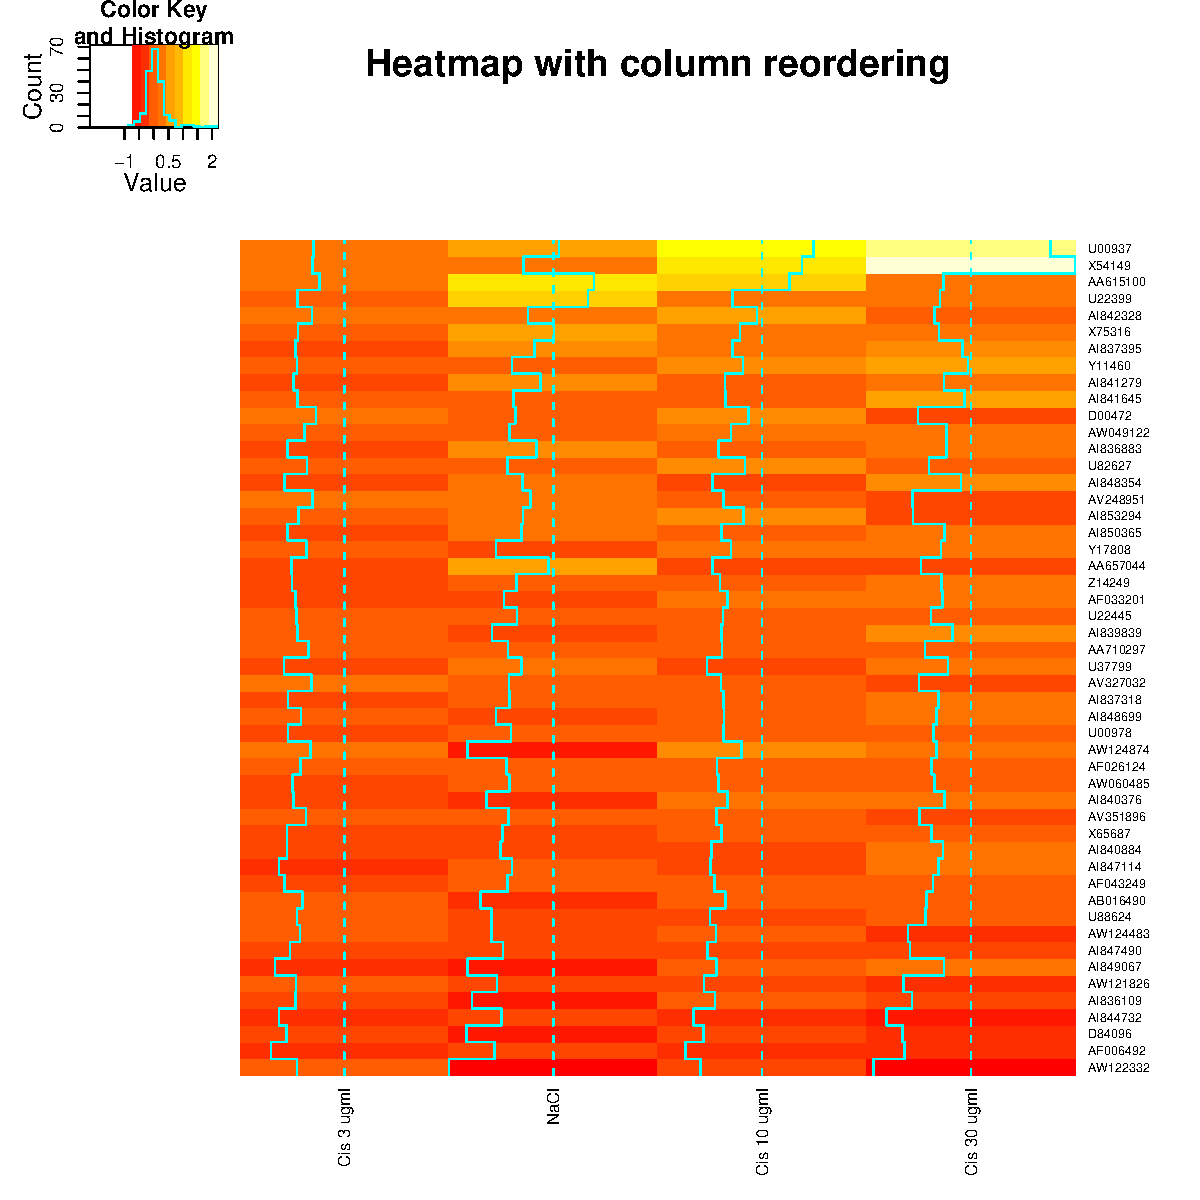
\includegraphics[width=\textwidth]{logDataColOrd}
\caption{Heatmap with column reordering}
\label{Heatmap with column reordering}
\end{minipage}
\hfill
\begin{minipage}[t]{2.5in}
\centering
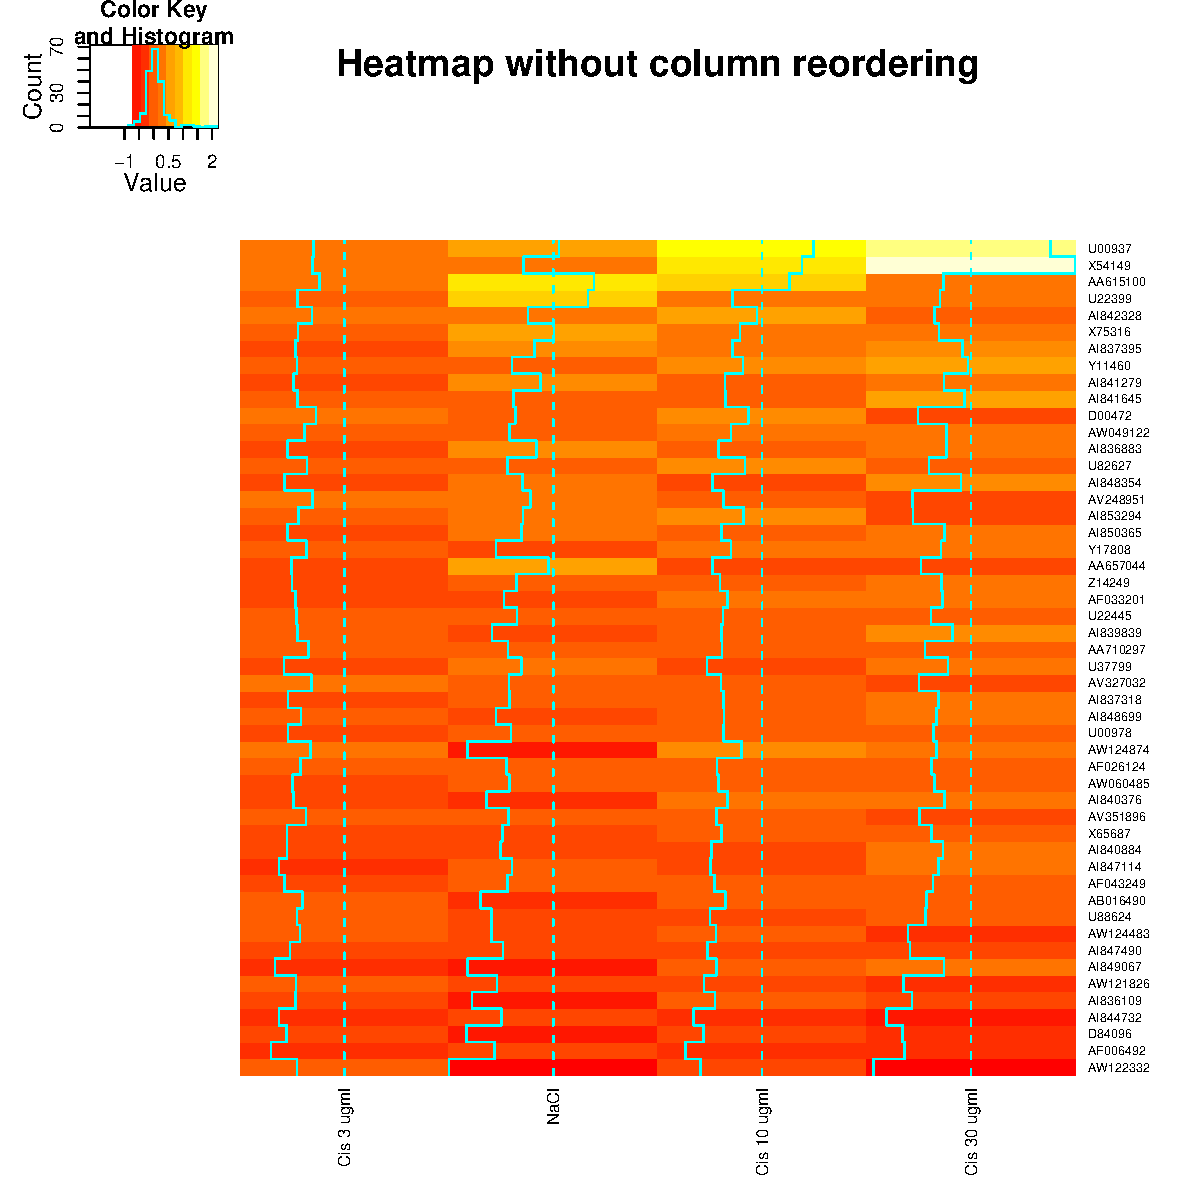
\includegraphics[width=\textwidth]{logDataColOrdNo}
\caption{Heatmap without column reordering}
\label{Heatmap without column reordering}
\end{minipage}
\end{figure*}

\subsection*{Ordering of rows and columns}
	This issue deals with whether and how the rows and columns
of the data should be reordered. Sometimes, rows and columns are
ordered to see the \textit{closeness} (based on some distance
metric) between the genes or treatment conditions.

%% Two figures corresponding to the rcolumn dendrograms - log data
\begin{figure*}[p]

\begin{minipage}[t]{2.5in}
\begin{center}
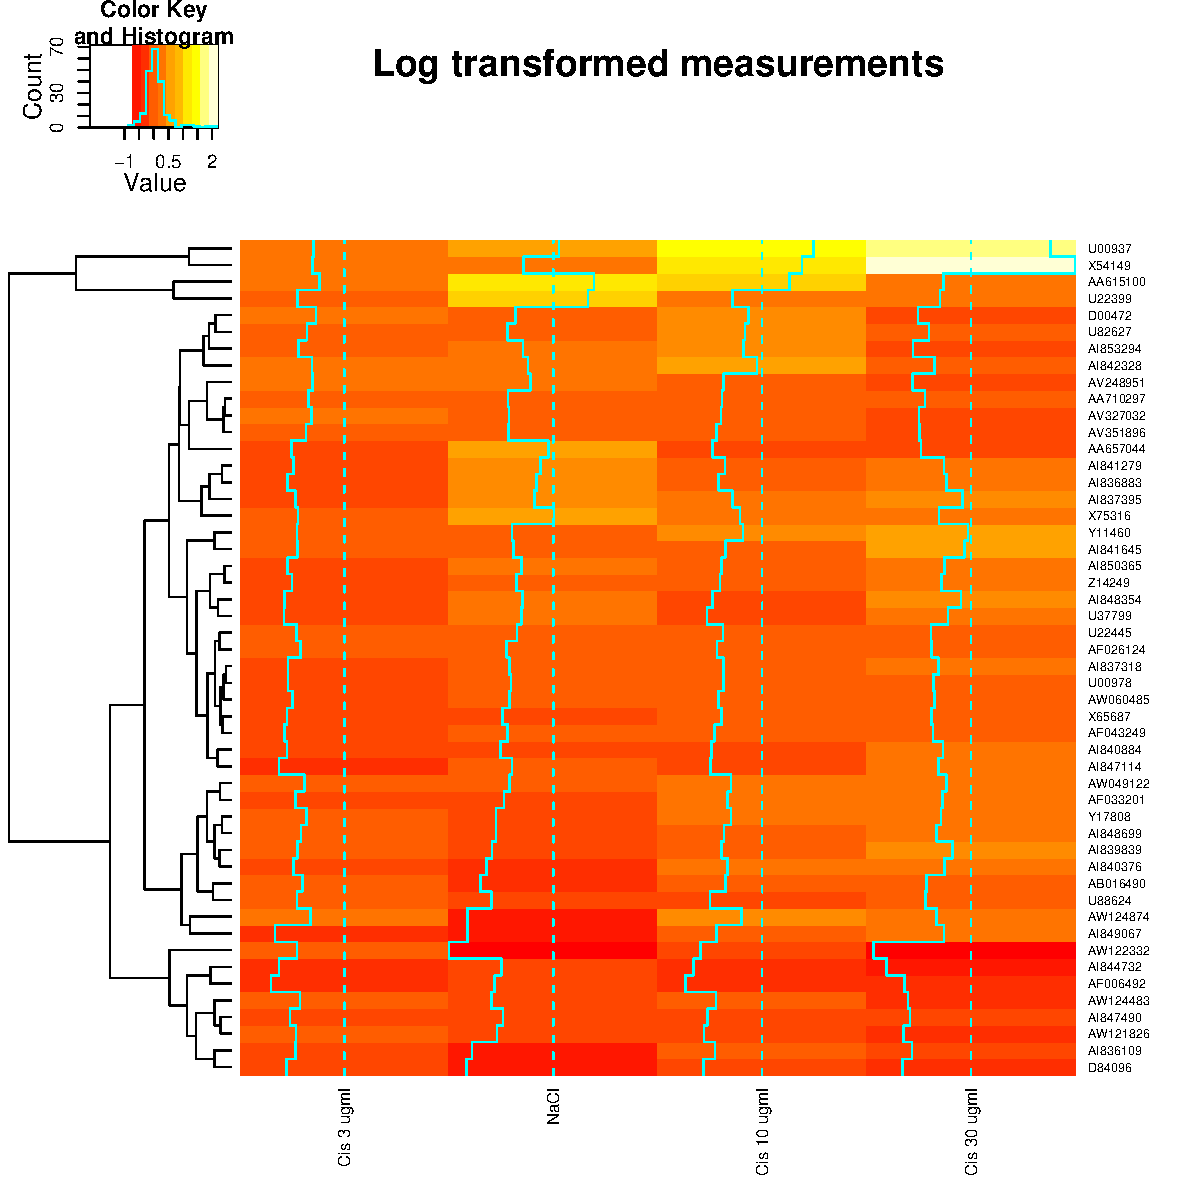
\includegraphics[width=\textwidth]{logDataRowDendrogram}
\caption{Log transformed measurements - Row dendrograms}
\label{Log transformed measurements - Row dendrograms}
\end{center}
\end{minipage}
\hfill
\begin{minipage}[t]{2.5in}
\begin{center}
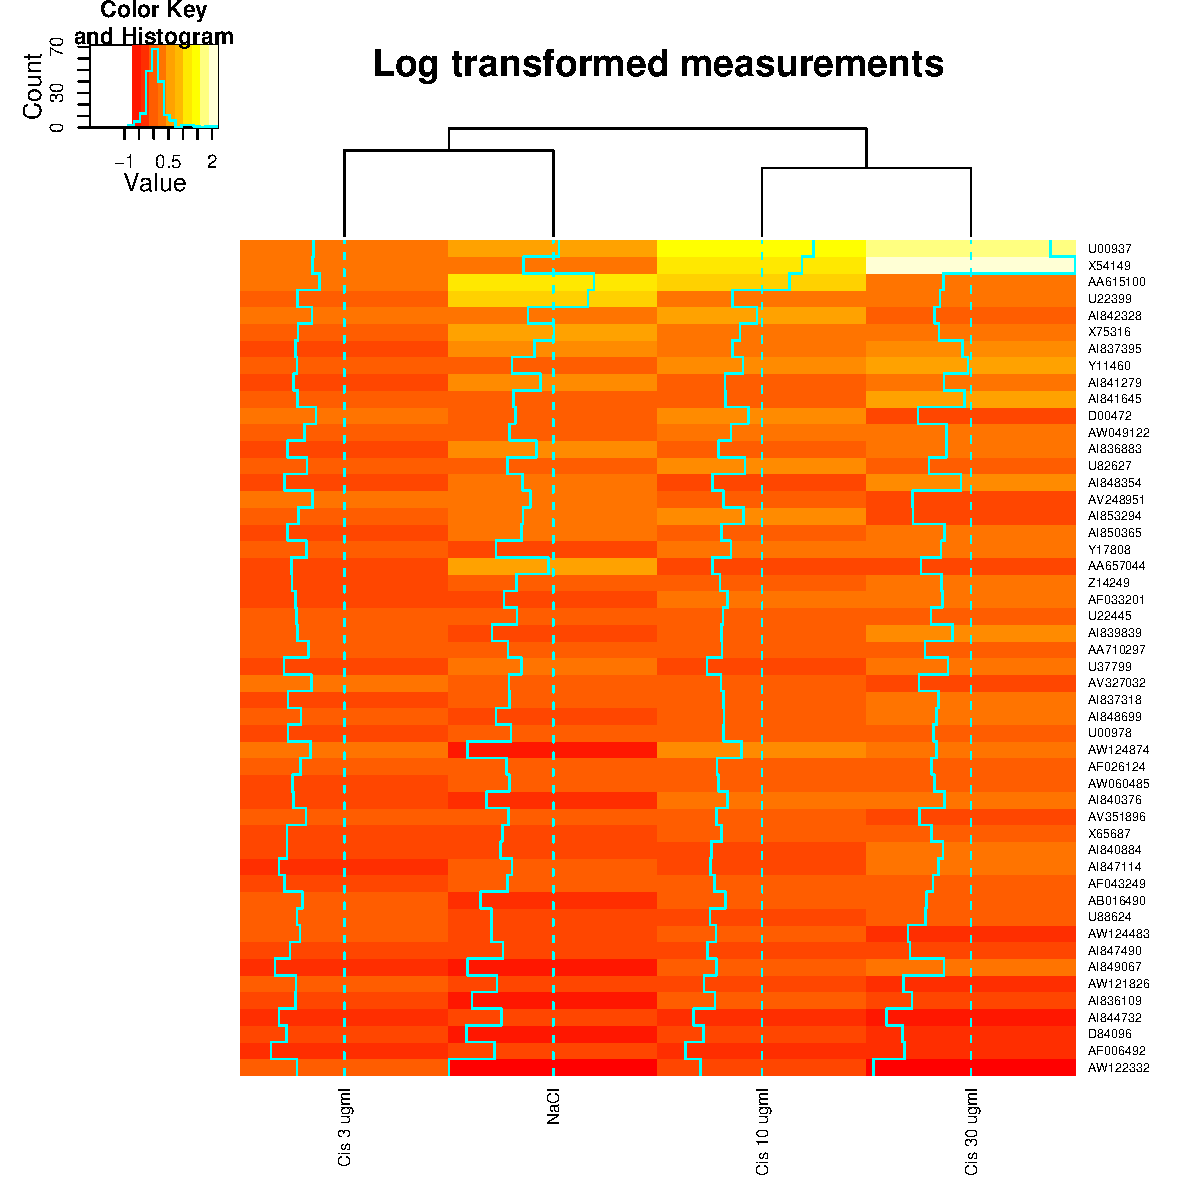
\includegraphics[width=\textwidth]{logDataColDendrogram}
\caption{Log transformed measurements - Column dendrograms}
\label{Log transformed measurements - Column dendrograms}
\end{center}
\end{minipage}

\caption{Heatmaps with row and column dendrograms}
\end{figure*}

\subsection*{Treatment effect estimates vs Raw data, i.e. Individual
	    values or summary representation} 
        Often people wonder about the relative merits of plotting
        treatment effects by combining the similar experimental
        conditions as one group and taking memedian to represent
        the expression levels in that group vs plotting individual
        conditions separately. The advantage of p;otting the raw
        data is that one can see the variability in the data but it
        is difficult to visualize the patterns.

\subsection*{Display Labeling and dendrograms}
	Heatmaps provide an option to display the x- and y-axes
labeling and the dendrograms along each axis. 
	
\subsection*{Choice of color}
	Shades or red, green and black have been accepted as
	`de-facto' colors in heatmap due to historic reasons as
	described above. While this color scheme is traditional, it
	is not optimal. On traffic signals, red indicates stop and
	green indicates go. However, in microarrays, red color is
	traditionally used to represent the up-regulated genes
	(i.e. genes with higher expression) and green color is used
	to represent down-regulated (lower expression). Moreover,
	the same intensities of red and green color are perceived
	differently by human eyes, with red color getting immediate
	attention~\cite{NaturePaper}.  Moreover, many people are color
	blind in differentiating between red and green. Red and
	green also sometimes give a false impression that elements
	indicated by red color are more important as red seems to be
	an eye-catcher. Alternative color combinations are to use
	shades of red and blue, or blue and yellow. Many people
	prefer shades of gray to convey the message, as it is
	independet of choice of colors.



\section*{Element, shape and separator}
	The elements in heatmap can be circle, rectangles, square or
	other shape, but typically the most common ones are
	rectangles.

\begin{figure*}[p]
\begin{minipage}[t]{2.5in}
\centering
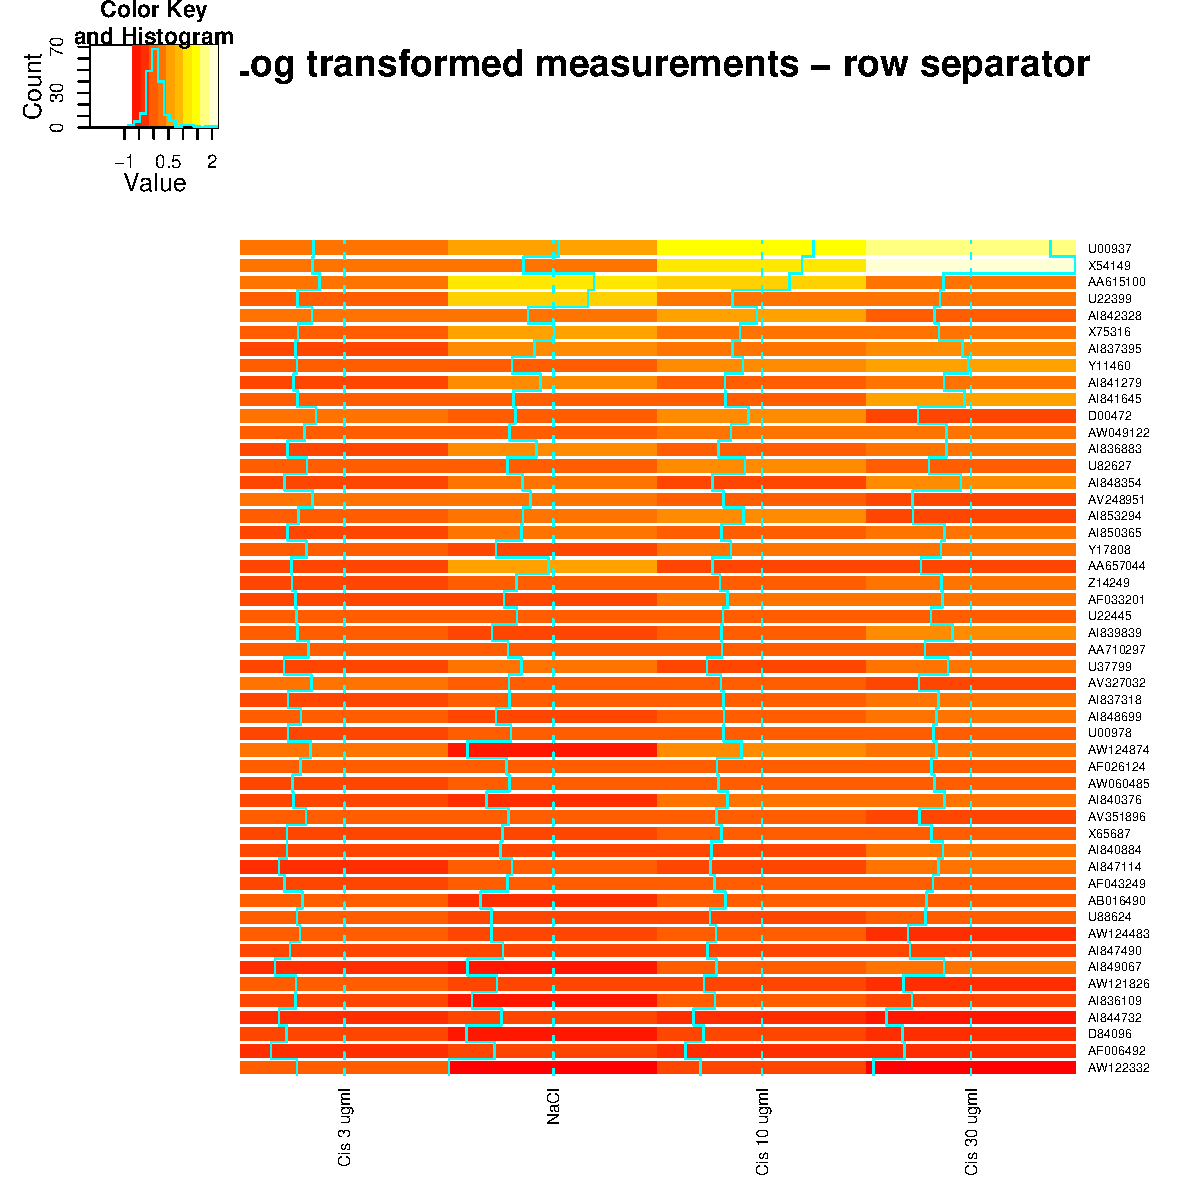
\includegraphics[width=\textwidth]{rowSeparator}
\caption{Row separated heatmap}
\label{Row separated heatmap}
\end{minipage}
\hfill
\begin{minipage}[t]{2.5in}
\centering
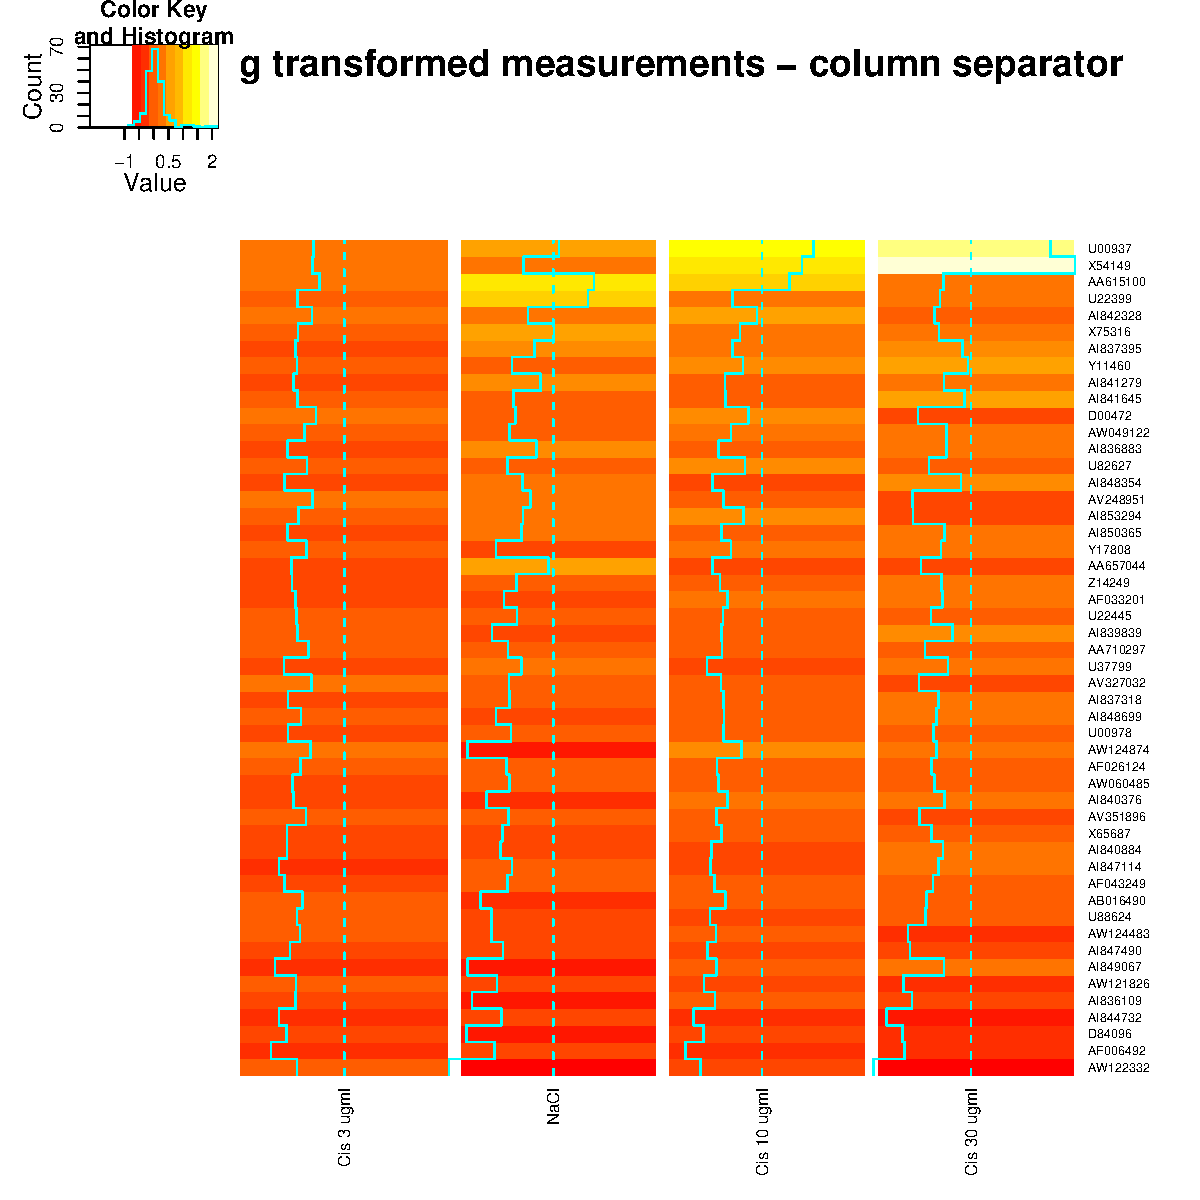
\includegraphics[width=\textwidth]{colSeparator}
\caption{Column separated heatmap}
\label{Column separated heatmap}
\end{minipage}
\end{figure*}


\section*{Choice of scales}
Data can be displayed in three formats thru heatmaps:


%% \use minipage to enter two figures side by side
%%
%%\begin{figure} 
%%\centering
%%\subfloat[]
%%{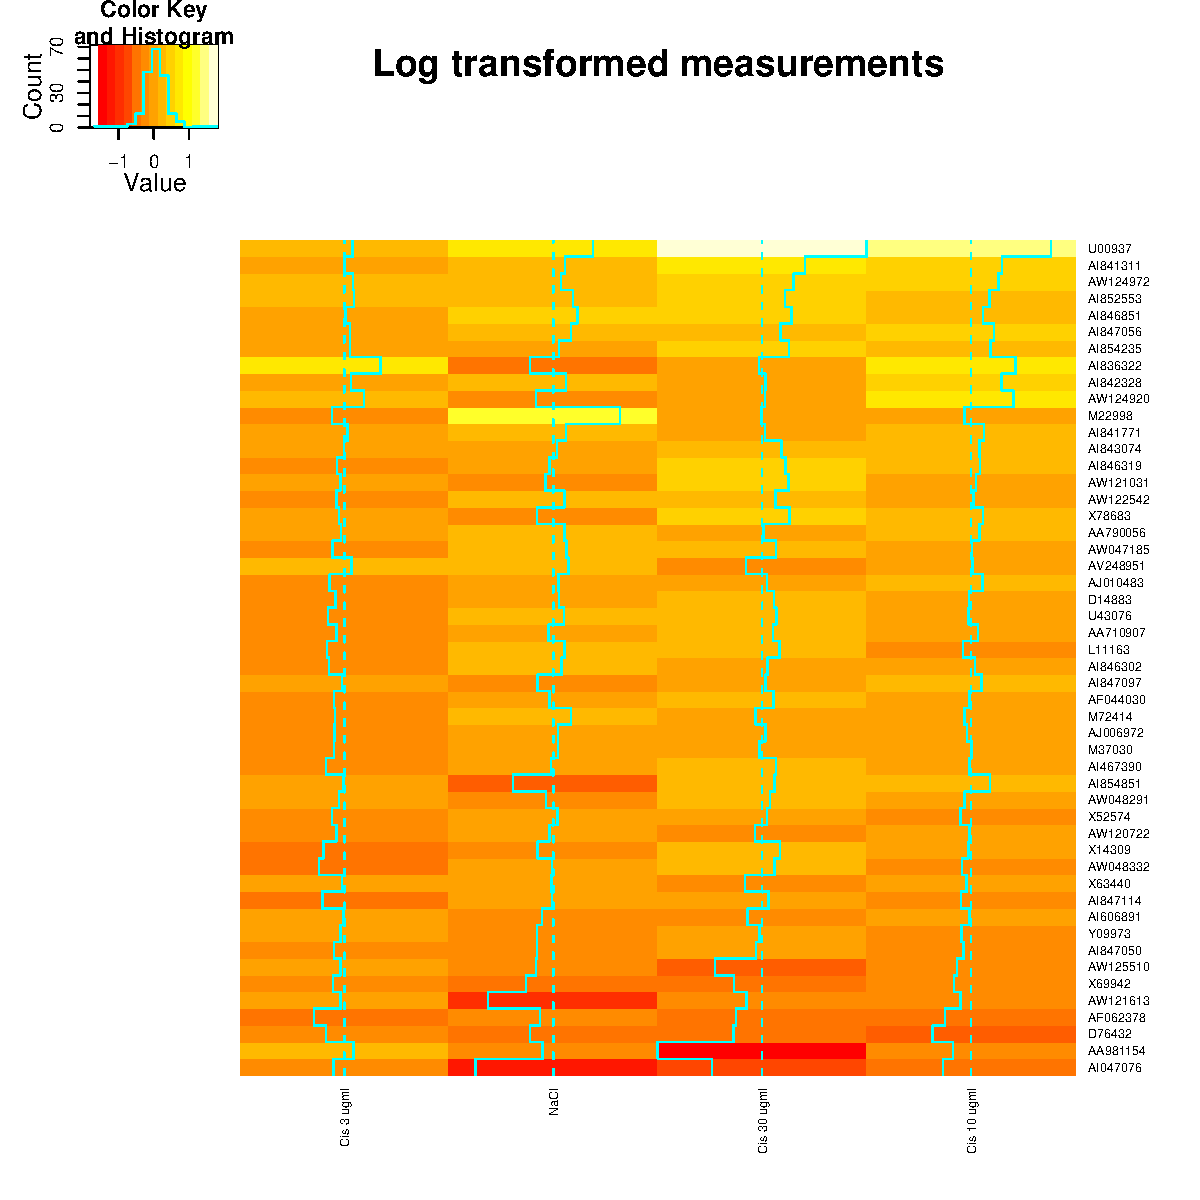
\includegraphics[width=\textwidth]{logData}
%%\label{test}
%%}
%%\subfloat[]
%%{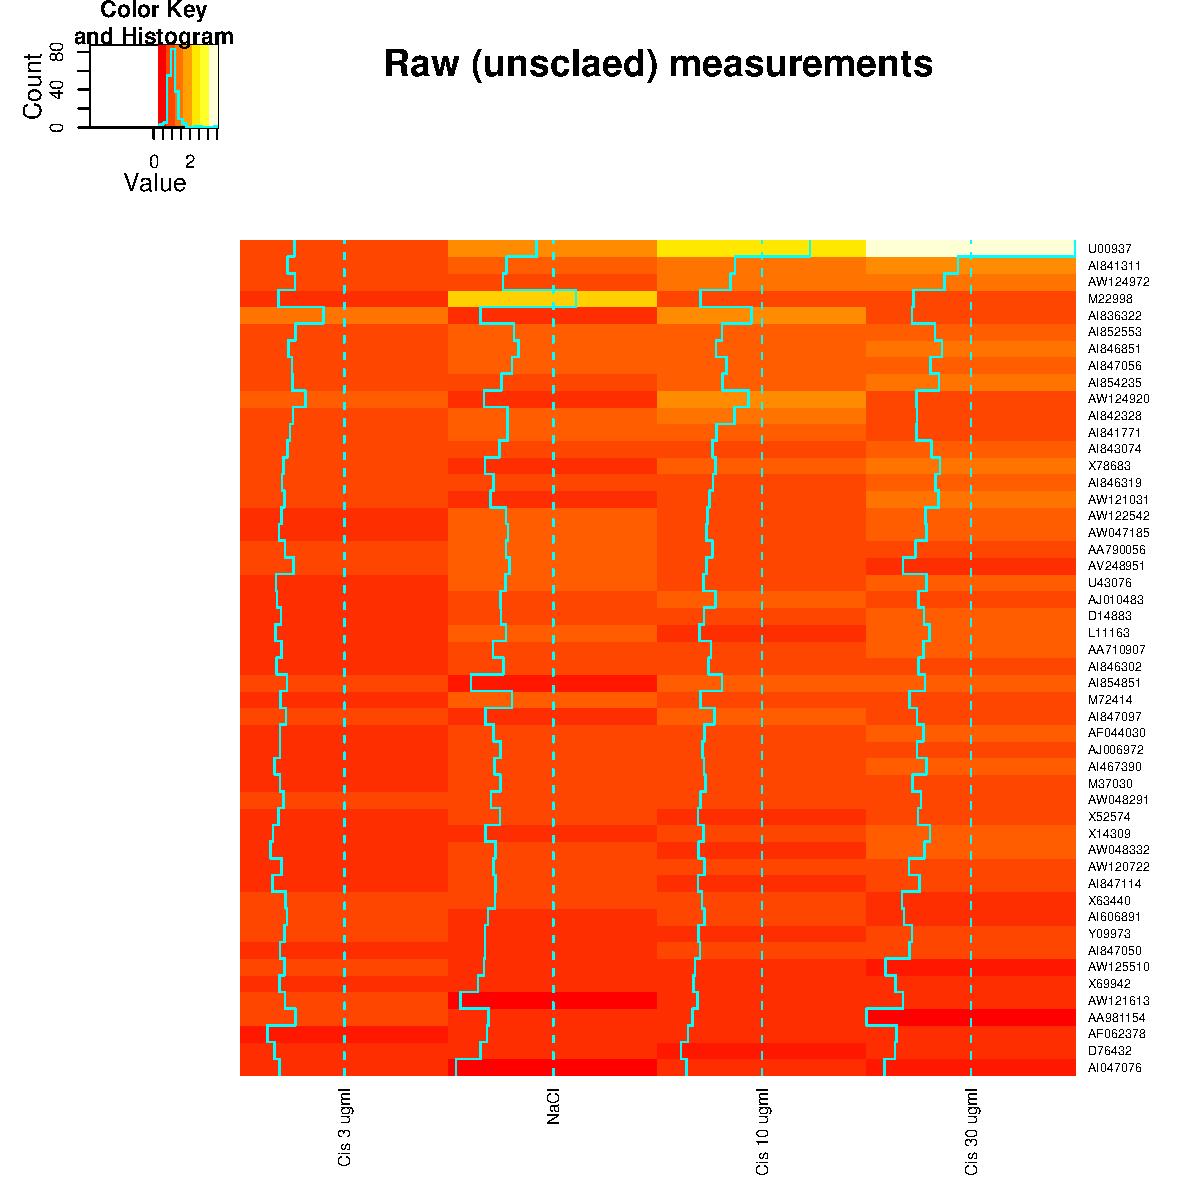
\includegraphics[width=\textwidth]{origScale}
%%\label{test2}
%%}
%%\caption{TESTING with subfigure}
%%\end{figure}
%%
%%





\begin{itemize}

\item {Log transformed intensities:} 
	This display is useful in finding which genes are expressed
	and which are not. However, this diplay has a drawback that
	if a few genes are expressed in very high amounts, they
	affect the display of rest of the genes by making them
	appear in similar shades of color.  Therefore, the visual
	interpretation of the clusters for most of the genes becomes
	difficult.

\item \textbf{Scaled intensities:} 
	In this display, the expression intensities of each gene is
	normalized across all the conditions (i.e. subtracted by
	mean and divided by the standard deviation). This display is
	useful in finding the patterns of the gene epression
	data. However, this method is also unable to differentially
	display the genes, if one gene is dominant in any one of the
	conditions.

%% Two figures corresponding to original scale-log scale data
\begin{figure*}[p]

\begin{minipage}[t]{2.5in}
\begin{center}
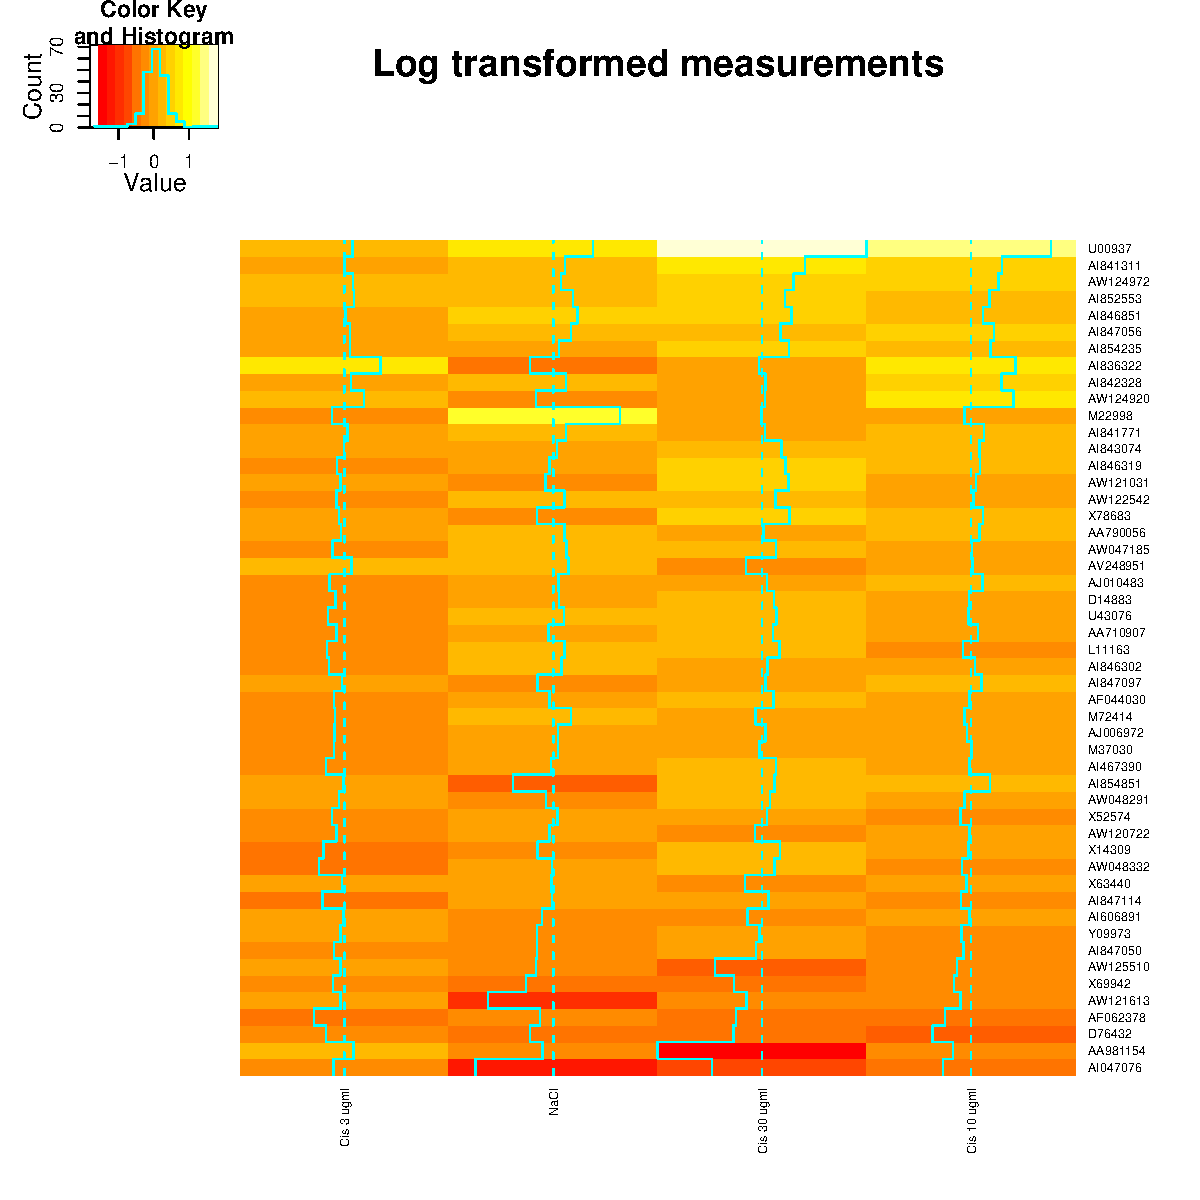
\includegraphics[width=\textwidth]{logData}
\caption{Log transformed measurements}
\label{Log transformed measurements}
\end{center}
\end{minipage}
\hfill
\begin{minipage}[t]{2.5in}
\begin{center}
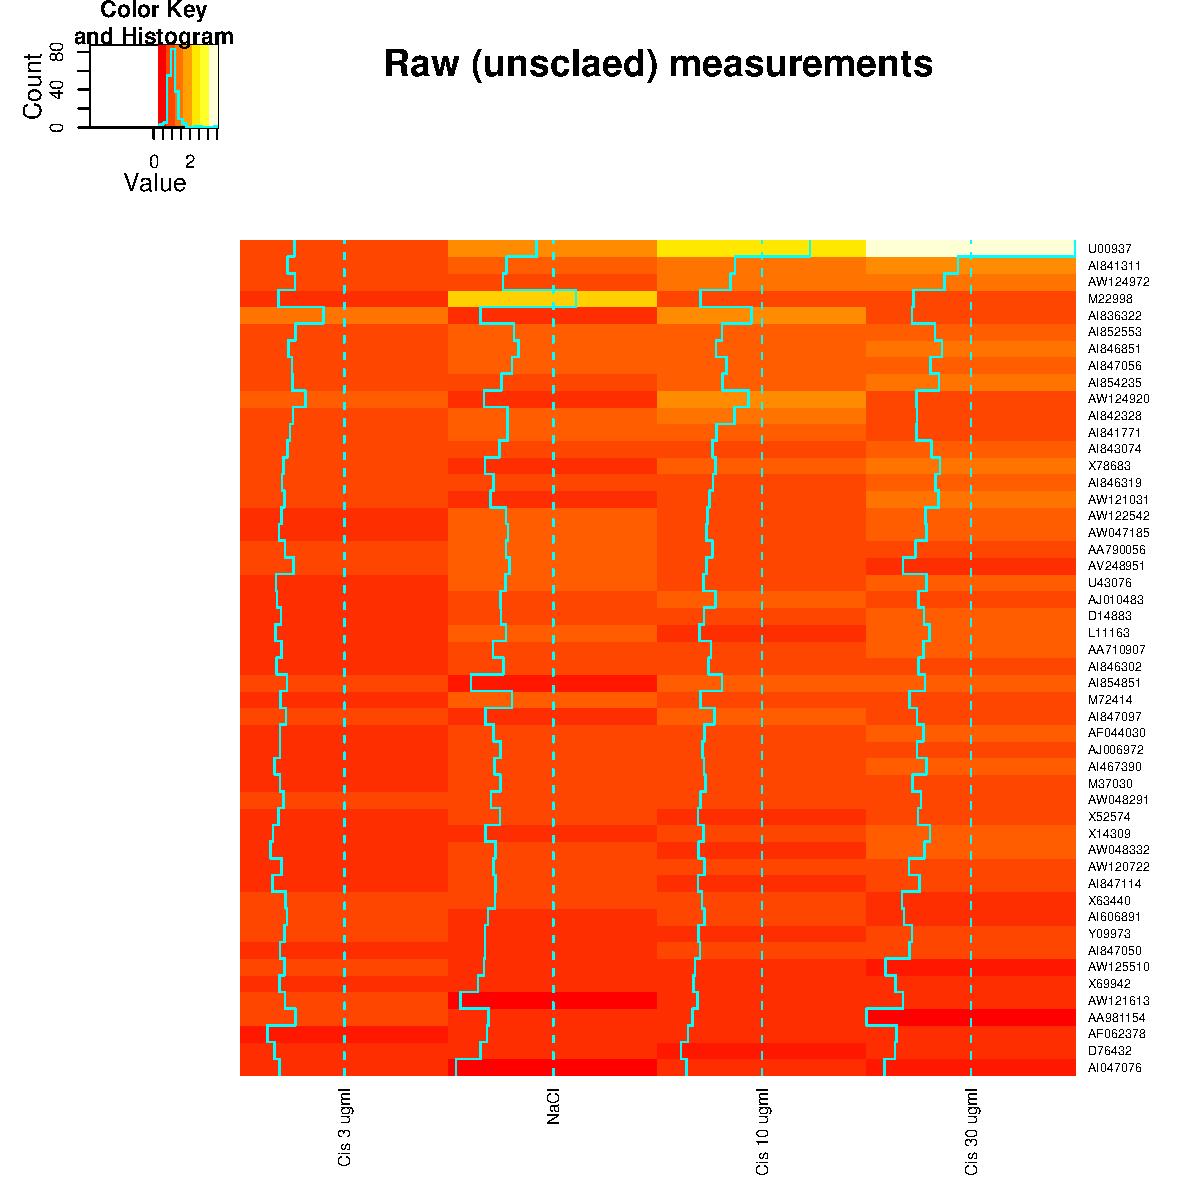
\includegraphics[width=\textwidth]{origScale}
\caption{Original scaled measurements}
\label{Original scaled measurements}
\end{center}
\end{minipage}

\caption{Different scales for the heatmap figure}
\end{figure*}



\begin{figure*}[p]
\begin{minipage}[t]{2.5in}
\centering
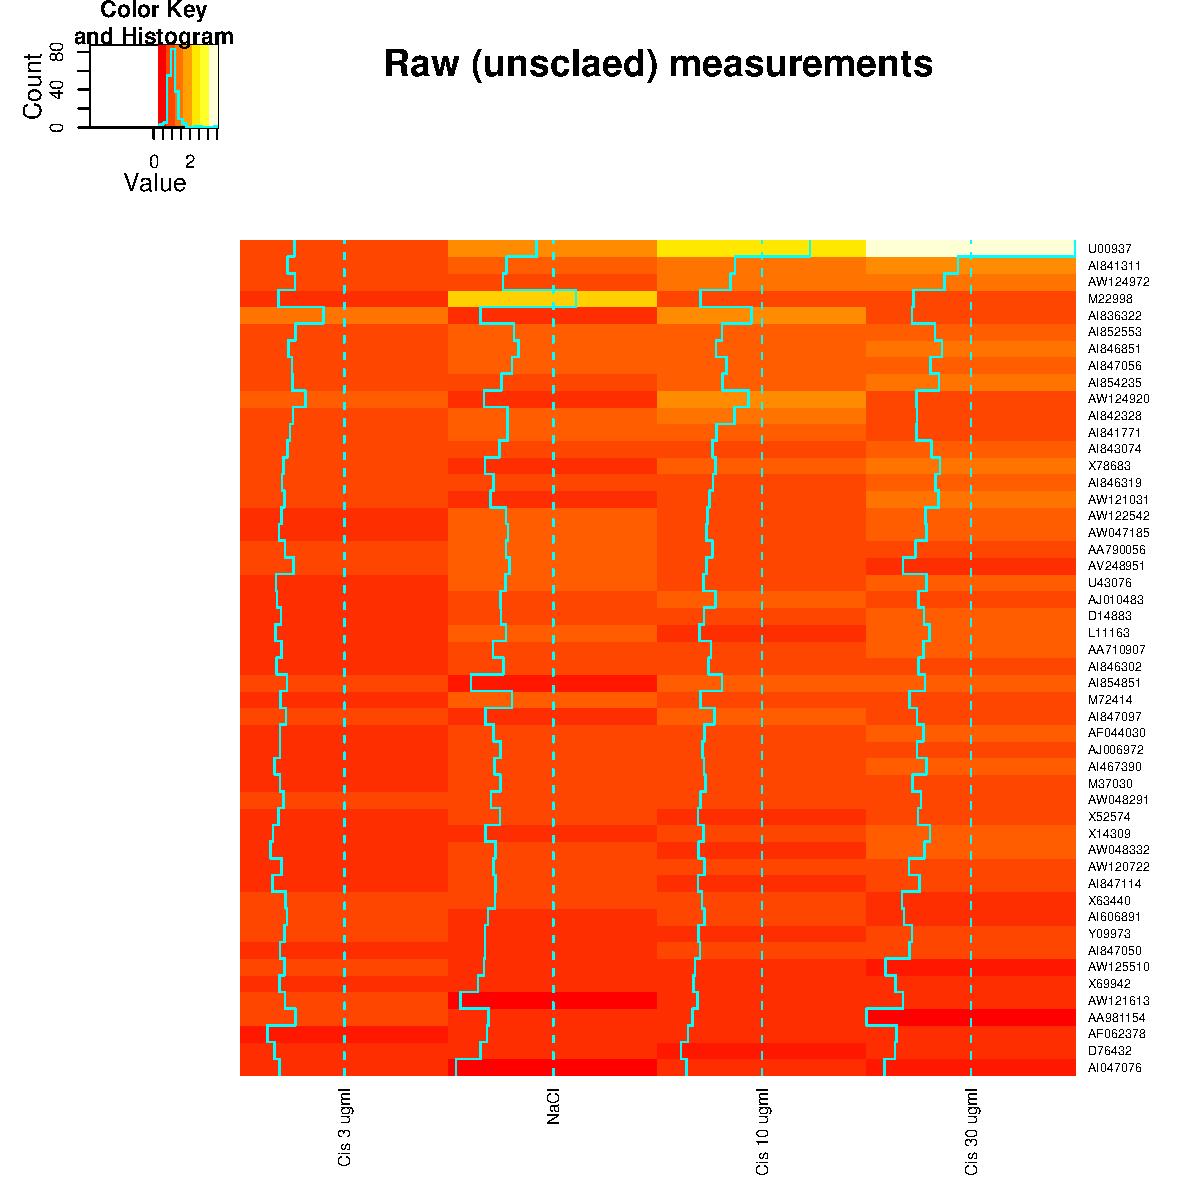
\includegraphics[width=\textwidth]{origScale}
\caption{Original scaled measurements}
\label{Original scaled intensities}
\end{minipage}
\hfill
\begin{minipage}[t]{2.5in}
\centering
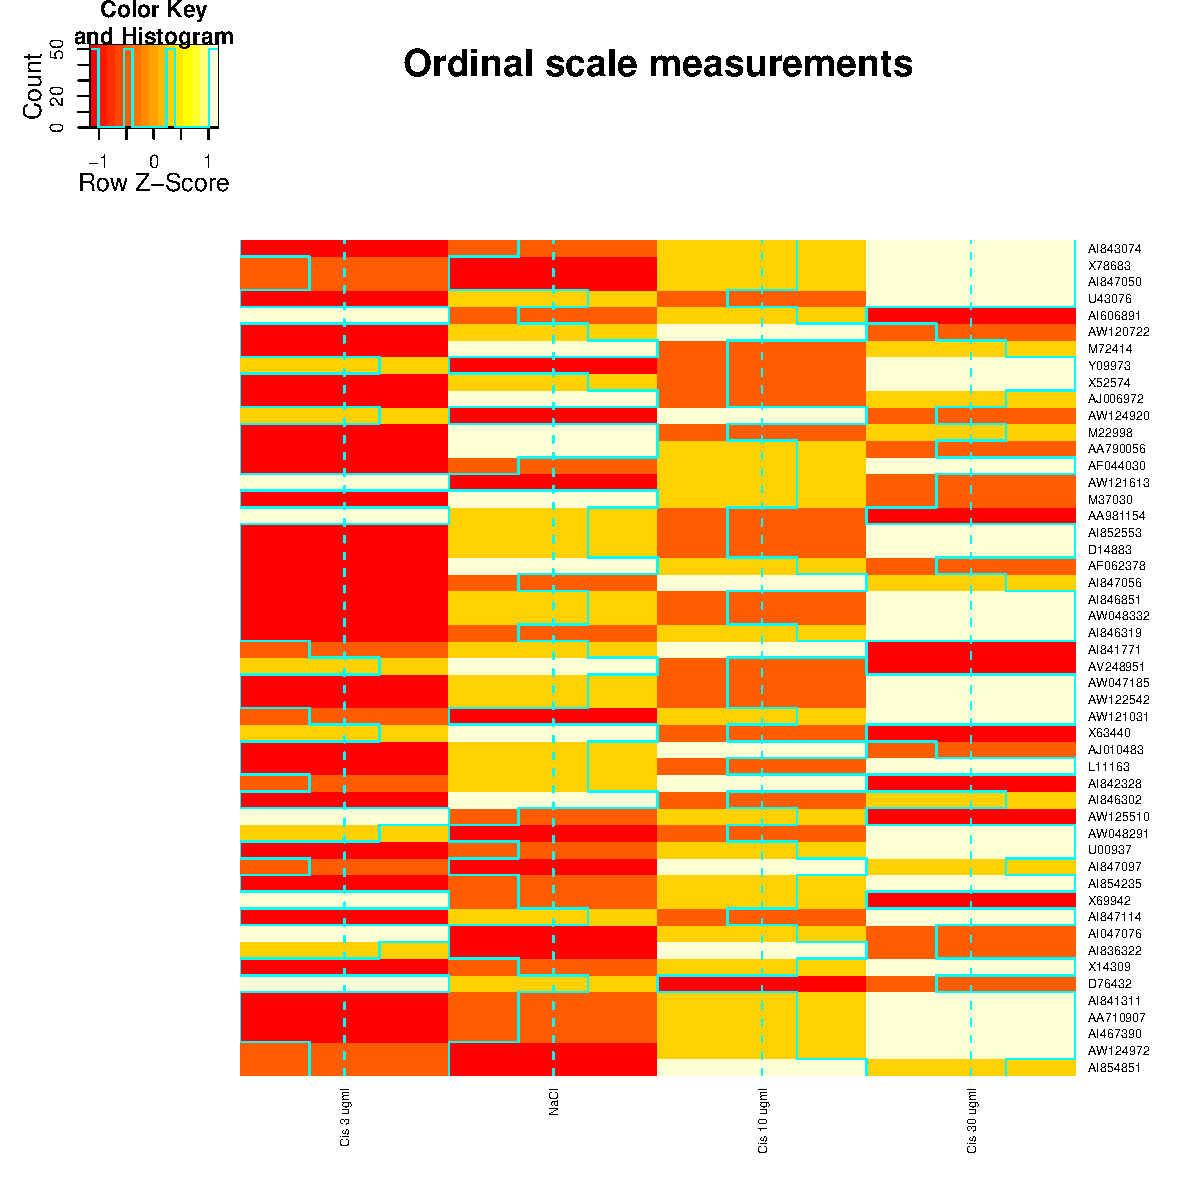
\includegraphics[width=\textwidth]{ordinal}
\caption{Ordinal scaled measurements}
\label{Ordinal scaled intensities}
\end{minipage}
\end{figure*}

\item \textbf{Ordinal Scale:}
	In this approach, each gene is ordered according to its
	expression values across different conditions. Hence each
	gene is assigned numbers from 1 to n (number of conditions)
	in different conditions, where 1 corresponds to the
	condition in which gene has lowest expression and n
	corresponds to the condition with highest expression. In
	heatmap, for each gene, the lowest order (i.e. 1) is
	displayed by brightest green, and highest order
	(i.e. `\textit{n}', where \textit{n} is the number of
	conditions) by brighest red, then the overall display
	becomes independent of the amount of expression of the gene.
	We name this display as `ordinal-scale'. This display is
	quite useful in finding the patterns of gene expression, as
	every gene possesses the same shades of color irrespective
	of the intensity.

\end{itemize}


	All the three approaches mentioned above have pros and cons
	and heatmaps from the above approaches should be interpreted
	together to get clear understanding.  While heatmaps based
	on $\log_2$ intensities give the overall picture of which
	genes are ovunder expressed, they often fail to visually
	convey the pattern of expression due to a few highly
	over-expressed genes. Heatmaps based on normalized intensity
	values are better in displaying the patterns, but they may
	also be misleading in conveying the information due to
	presence of highly over-expressed genes.  The heatmaps based
	on the proposed ordinal scale method effectively capture the
	patterns of gene expression, and are un-effected due to the
	presence of highly expressed genes. However, heatmaps based
	on ordinal scale especially overestimate small differences
	in gene expression.  Therefore, all heatmaps (especially
	$\log_2$ and ordinal scale) should be investigated
	carefully.

\section*{Heatmap extensions}

	In order to differentiate between different shades of color,
	we hae developed ``heatmap.2'', which provides some
	additional features. One of the most common problems in the
	original heatmap is the difficulty to distinguish bewtween
	different shades of color. To address this issue,
	\textit{heatmap.2} provides an option of drawing a trace
	line across rows or columns or both. The distance of the
	line from the center of each color-cell is proportional to
	the size of the emasurement. Default color of the trace line
	is cyan.

Heatmap.2 also provides and option to draw a color-key. Density plot
or histogram can be added to the color-key in order to improve the
legibility of the key.

Heatmap.2 also provides an option to display statistically
significant objects by different characters such as *, and different
models used by other symbols..
	



\section*{Limitations of heatmaps}
	Hierarchical clustering suffers from a number of pitfalls -
	depending on the choice of distance metric, different
	results are obtained. It is not unique, and may give
	different results in case of ties (i.e. same correlation
	between more than two groups).

	Sometimes people mistake the proximity between the
	dendrograms for their closeness in the cluster. However, one
	must understand that the two branches from a parent node in
	a heatmap act like hinge, they can be flipped easily without
	any change in menaning. Distance between two objects in a
	heatmap is directly proportional to the height of the
	dendrograms by which they are joined.


\section*{Recommendataions}

	The choice of scale is quite important - we believe that
	ordinal scale is best suited for displaying the patterns. If
	the aim of the heatmap is to visualize variability in the
	data, then all the experimental conditions should be used to
	display the heatmap. However, if the aim is to identify the
	patterns in the data, then similar groups should be combined
	in one by mean or median statistics.

   	We believe that blue-white-yellow color scheme
   	is better than red-black-green or black-grey-white
   	scheme. 

	The contiguous rectangles are most traditional and common
	ways for displays in heatmap and are just fine. Further
	research is needed for effects of shape, elements and
	separator on human perception.


\section*{Discussions}

	Despite some of the pitfalls of displaying gene-expression
	data by heatmaps, they are one of the most common choices
	currently available. All the three methods of display (based
	on absolute intensity, scaled intensity or ordinal scale)
	should be considered together to make inferences from the
	data.


\begin{thebibliography}{99}

\bibitem{Eisen1998} Eisen, M.B., Spellman, P.T., Brown, P.O., and
Bolstein, D. (1998) ``Cluster analysis and display of genome-wide
expression patterns'', \textit{Proc Natl Acad Sci USA} 95, 14863-14868.

\bibitem{heatmap}   Liaw, A., Gentleman, R., Maechler, M. and  Huber, W.
``Heatmap function in stats package in R''. \textit{(htt/cran.r-project.o)}

\bibitem{OrigPaper} Dickinson, D.A., Warnes, G.R., Quievryn, G., Messer, J.,
Zhitkovich, A., Rubitski, E., and Aubrecht, J. (2004) ``Differentiation of
DNA-reactive and non-reactive genotoxic mechanisms using gene
expression profile analysis'', \textit{Mutation Research}, Volume 549, Issues
1-2, pp 29-41.


\bibitem{NatuerPaper} Holcombe A.O., and Cavanagh, P. (2001) ``Early
binding of feature pairs for visual perception'' \textit{Nature Neuroscience},  4, 127 - 128.




\end{thebibliography}

\end{document}



